%% The following is a directive for TeXShop to indicate the main file
%%!TEX root = diss.tex

\chapter{Background}
\label{ch:Background}

\section{BDI}
\label{sec:BDI}
The BDI cache introduced in \cite{bdi} is a cache that takes advantage of similarities within data lines to compress those lines into smaller sizes. In the following section we discuss the BDI cache, it's compression, structure, and operation.
\subsection{Compression}
\label{Compression}
\subsubsection{Base Delta Compression}
\begin{figure}
    \makebox[\textwidth][c]{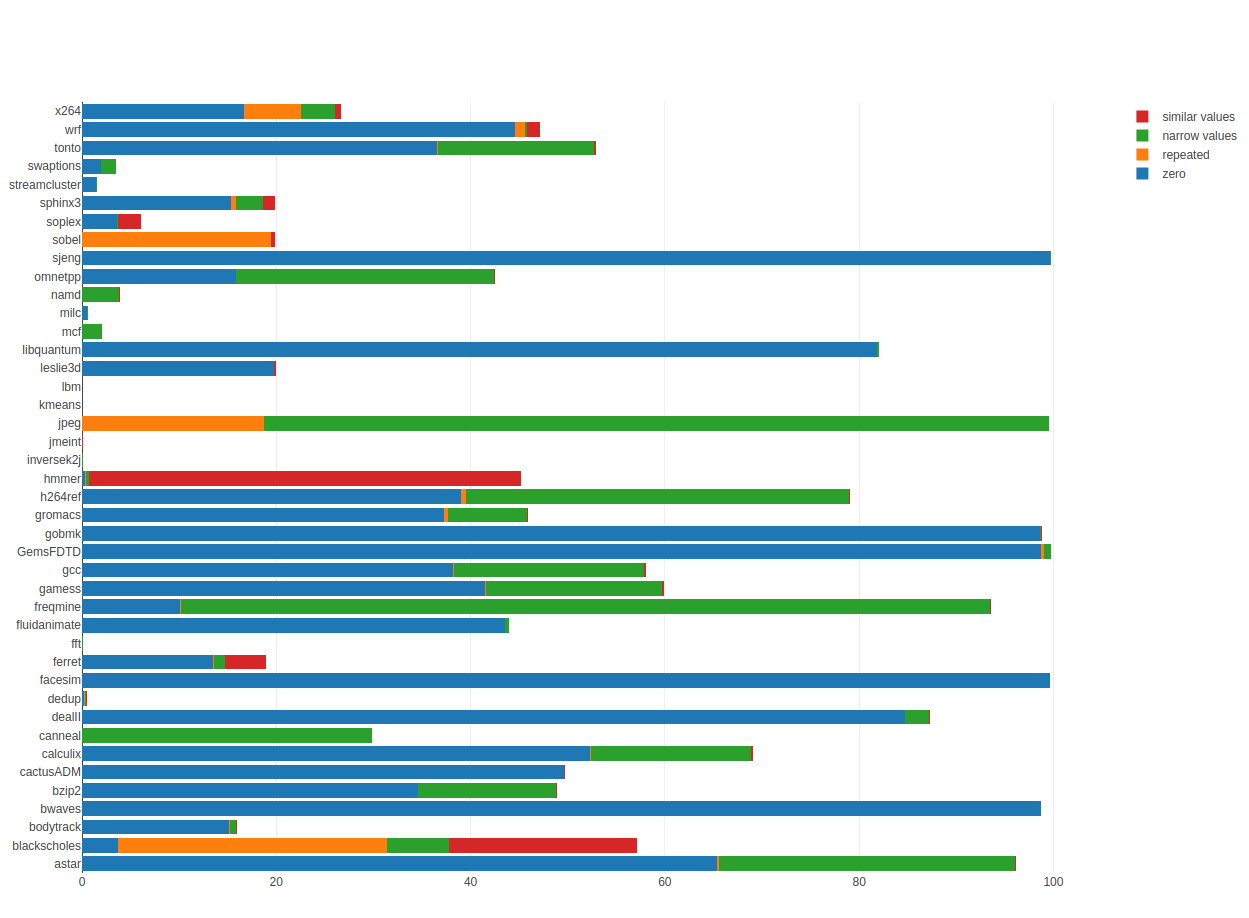
\includegraphics[width=1.5\textwidth]{BDIPotential.png}}
    \caption[BDI Patterns]{The figure shows the percentage of cache lines that have one of the following patterns: zero, repeated values, narrow values, or near values. Recreated from \protect\cite{bdi}}
    \label{fig:BDIPotential}
\end{figure}
The authors in \cite{bdi} have observed that data lines of real world applications have a great degree of redundancy, some of the patterns observed are:
\begin{itemize}
    \item \textbf{Zeros:} A lot of cache data lines are zeros, this is a very common case because zeros are usually used to initialize data structures, they're also very common in applications that deal with sparse matrices.
    \item \textbf{Repeated Values:} This can be observed in applications that initialize large arrays to the same initial value, or in multimedia applications where adjacent pixels could hold the same colours.
    \item \textbf{Narrow Values:} Programmers typically code for the worst case and thus have to pick larger data types while the majority of the values can fit in smaller narrower data types.
    \item \textbf{Near Values:} Values that are somewhat similar but not exactly, those are values that have high entropy in their lower bits but have the same higher bits. An example would be a list of pointers that are in the same memory regions, or pixels of an image that have almost similar colours.
\end{itemize}
Figure \ref{fig:BDIPotential} shows the percentage of lines where those patterns occur in a cache.\par
In the previously mentioned patterns, the data in a cache line granularity have a low dynamic range, the difference between values in one cache line can be represented using fewer bytes than the original data type. A compression scheme was proposed to utilize this low dynamic range. It works by representing the data line using a base value, and an array of delta values. Since the delta values can be smaller in size than the original data elements, this allows for a lot of savings in the data line itself. If the delta size required to represent the delta is not smaller than the original size, the line is then not compressible and is left untouched.\par
Finding the right base is key to compress the data line optimally, and it happens in two steps:
\begin{itemize}
    \item \textbf{Finding the base size:} The right base size would affect the deltas and their sizes, and thus will affect the final compression size. Since caches have no knowledge of the data types stored in them, compression is not able to identify whether a specific data line is comprised of 16 bit integers or 32 bit floats and so the base size is not directly known. Choosing one base size statically would greatly reduce the opportunity for compression, so the authors opted to allow three different base sizes: 2, 4 and 8 bytes that can used simultaneously and the one that provides the best compression should be used.
    \item \textbf{Finding the base value:} Once a base size is chosen, the base value itself mush be found. Ideally, selecting the base value in a compressed line should be in the middle point between the minimum and the maximum values of a cache line. To avoid the hardware implementation complexity of finding the base, the authors opted to use the first value as base.
\end{itemize}
The allowed compression schemes and compressed sizes are shown in Figure \ref{fig:BaseDeltaCompression} and table \ref{tab:BDICompressionSizes}.
\begin{figure}
    \makebox[\textwidth][c]{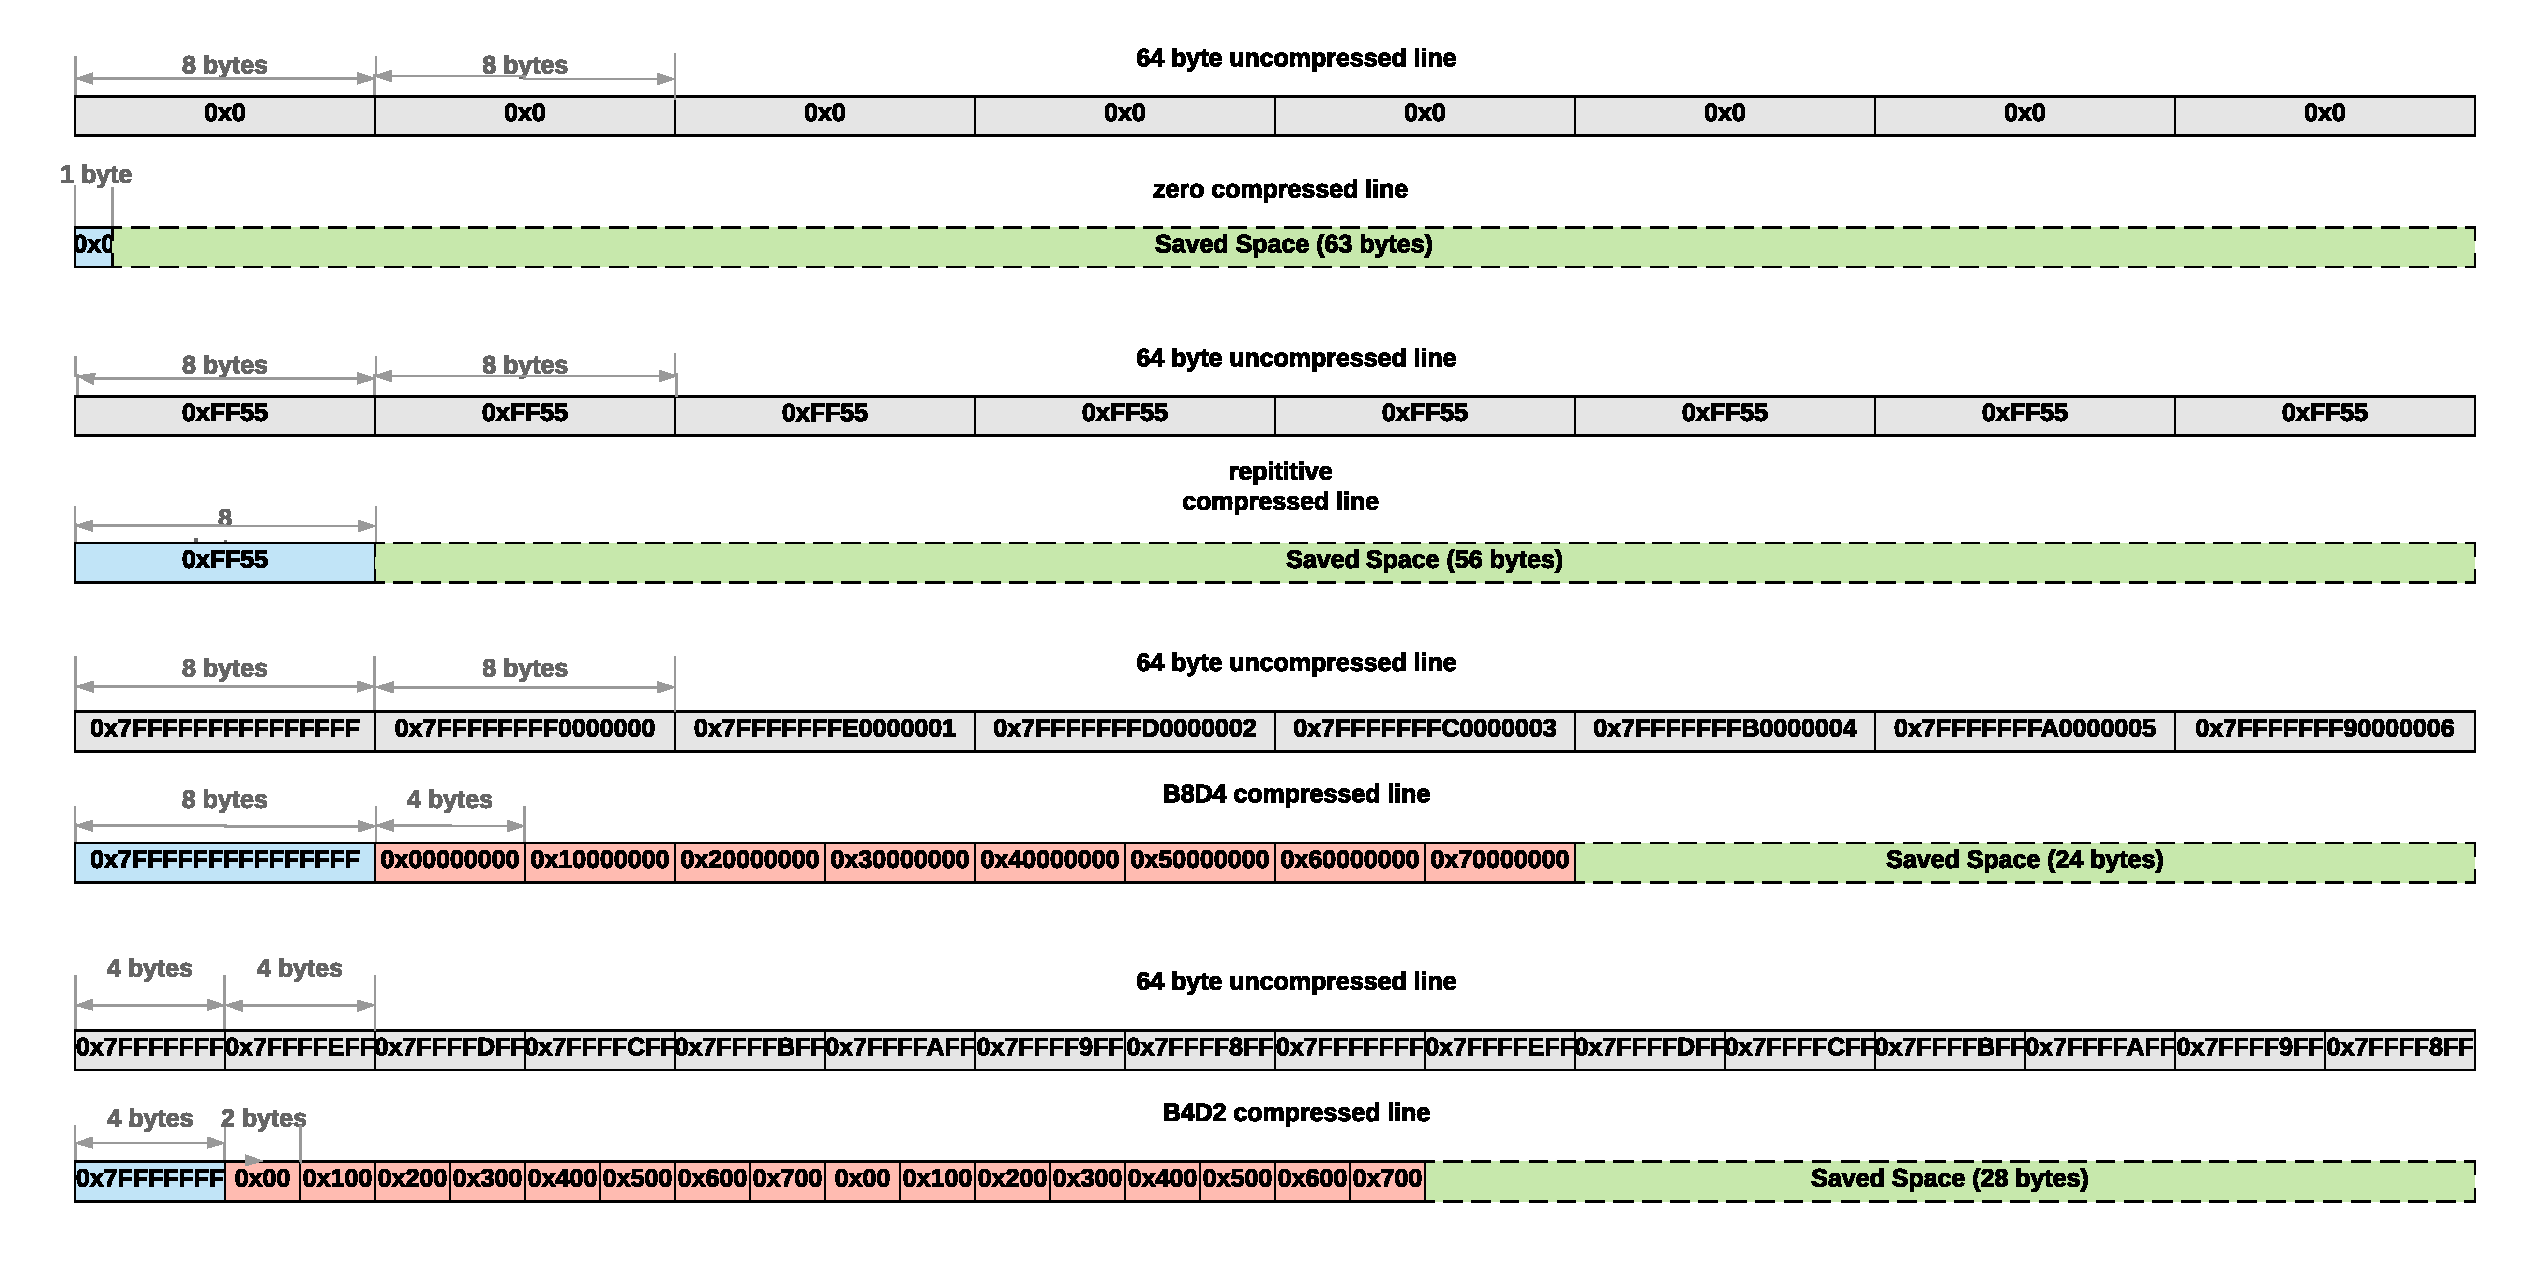
\includegraphics[width=1.5\textwidth]{BaseDeltaCompression.pdf}}
    \caption[Base Delta Compression Examples]{The figure shows examples of different cases of Base Delta compression.}
    \label{fig:BaseDeltaCompression}
\end{figure}
\subsubsection{Base Delta Immediate Compression}
Although one can gain a lot of compression from the base delta compression scheme, some patterns cannot be represented just by one base value. An example would be applications that use structs comprising of different data types. Because of this, allowing the base delta compression to use more than one base might help compress such lines. Based on experiments in \cite{bdi} it was clear that bases more than two do not provide much compression, so the authors selected two bases as their optimum number. To avoid the complexity of looking for a second base when compressing a data line, the authors opted to use the second base as an implicit zero. The intuition behind this is when structs are used in applications, they're likely to contain wide values with low dynamic range (e.g. Pointers) along with narrow values, the authors observe that using an implicit zero base captures most of the compression enabled by using an arbitrary second base.
\begin{table}[]
\centering
\caption[BDI Sizes]{The table shows BDI compression sizes, all sizes are in bytes. Original line size is 64 bytes.}
\label{tab:BDICompressionSizes}
\begin{tabular}{|c|c|c|c|c|}
\hline
\textbf{Name}         & \textbf{\begin{tabular}[c]{@{}c@{}}Base\\ Size\end{tabular}} & \textbf{\begin{tabular}[c]{@{}c@{}}Delta\\ Size\end{tabular}} & \textbf{\begin{tabular}[c]{@{}c@{}}Compression\\ Size\end{tabular}} & \textbf{\begin{tabular}[c]{@{}c@{}}Compression\\ Encoding\end{tabular}} \\ \hline
\textbf{Zero}         & 1                                                            & 0                                                             & 1                                                                   & 0000                                                                    \\ \hline
\textbf{Rep}          & 8                                                            & 0                                                             & 8                                                                   & 0001                                                                    \\ \hline
\textbf{B8D1}         & 8                                                            & 1                                                             & 16                                                                  & 0010                                                                    \\ \hline
\textbf{B8D2}         & 8                                                            & 2                                                             & 24                                                                  & 0011                                                                    \\ \hline
\textbf{B8D4}         & 8                                                            & 4                                                             & 40                                                                  & 0100                                                                    \\ \hline
\textbf{B4D1}         & 4                                                            & 1                                                             & 20                                                                  & 0101                                                                    \\ \hline
\textbf{B4D2}         & 4                                                            & 2                                                             & 36                                                                  & 0110                                                                    \\ \hline
\textbf{B2D1}         & 2                                                            & 1                                                             & 34                                                                  & 0111                                                                    \\ \hline
\textbf{Uncompressed} & N/A                                                          & N/A                                                           & 64                                                                  & 1111                                                                    \\ \hline
\end{tabular}
\end{table}
\subsubsection{Compression Hardware}
\label{sssec:BDICompressionHardware}
The compression hardware used for BDI consists of eight units that operate simultaneously in parallel, two for the zero and repetitive compression schemes and six units for the three different bases with their deltas. Each unit corresponds for one of the compression sizes described in Table \ref{tab:BDICompressionSizes}. Each unit outputs whether the line can be compressed in its scheme or not, and if it can be compressed it also outputs the compressed line. If multiple units can compress the line then the selection logic picks the one with the least compressed size.
A compression unit treats the line as elements of its corresponding base size. It picks the first element as the base and then subtracts all the elements from the it. If all the results can be represented in the required delta size then the line is compressed. Figure \ref{fig:BDIHardware} shows the compression hardware.
\begin{figure}
    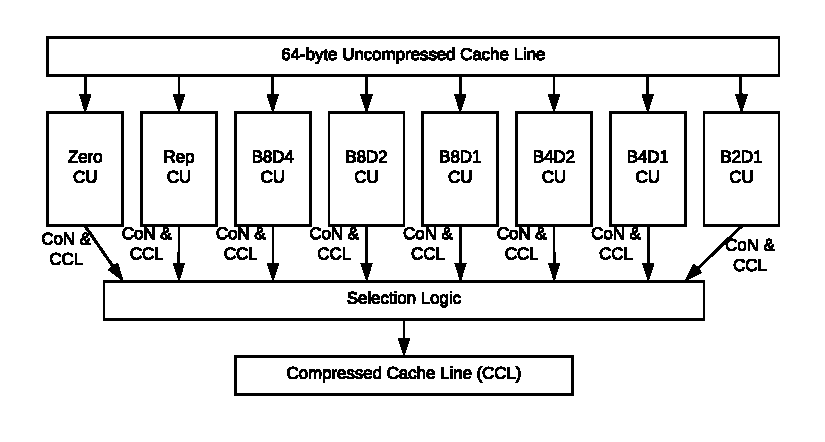
\includegraphics[width=\textwidth]{BDIHardware.pdf}
    \caption[BDI Compression Hardware]{The figure shows BDI compression hardware. CU: Compression Unit, CoN: Compressed or Not?, CCL: Compressed Cache Line. Recreated from \protect\cite{bdi}}
    \label{fig:BDIHardware}
\end{figure}

\subsection{Structure}
\label{ssec:BDIStructure}
\begin{figure}
    \makebox[\textwidth][c]{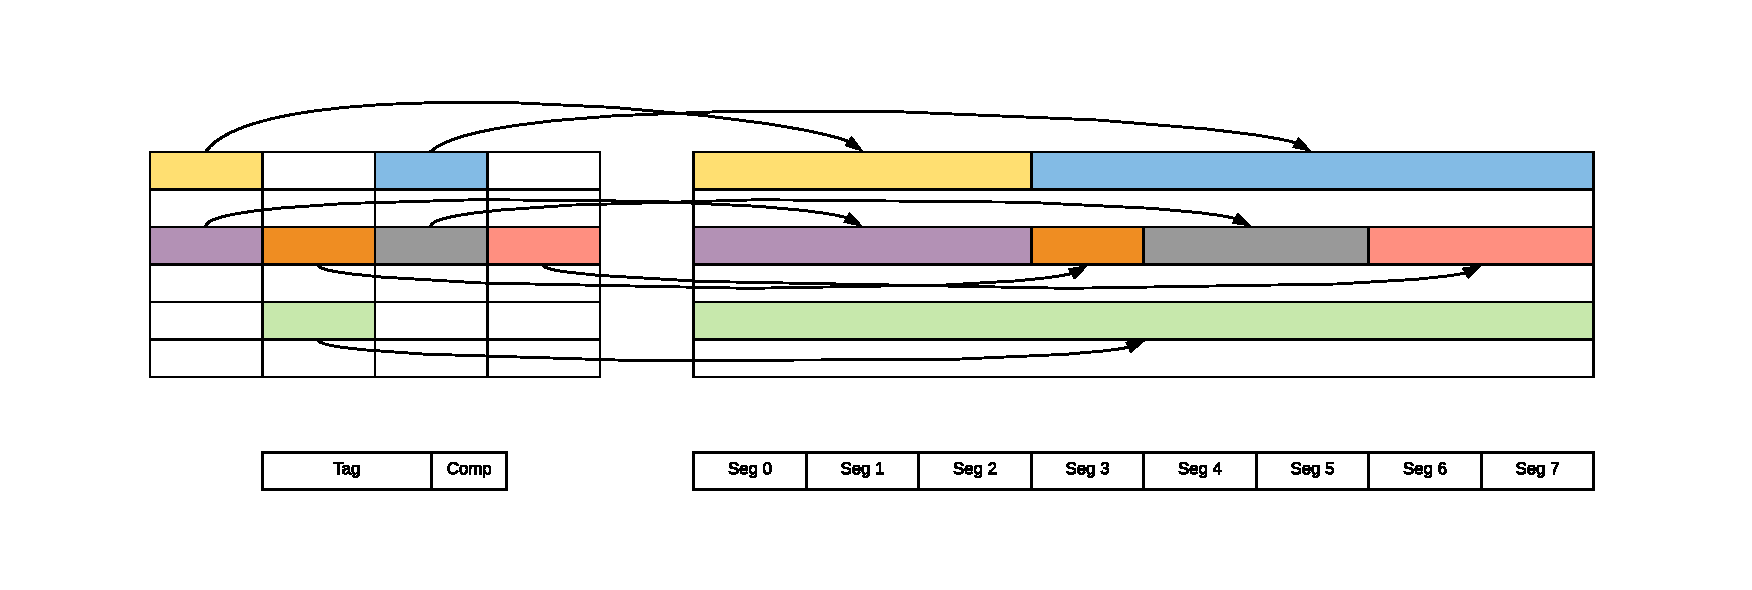
\includegraphics[width=1.5\textwidth]{BDI.pdf}}
    \caption[BDI Cache]{Conventional vs BDI, showing one set of each. Tags doubled, Data size same but divided to segments.}
    \label{fig:BDI}
\end{figure}
The BDI cache builds upon the conventional cache design by adding some modifications to allow compression. Tag and data arrays are arranged in sets, and tag sets and data sets are coupled. The BDI cache structure is shown in Figure \ref{fig:BDI}
\subsubsection{Tag Array}
\label{sssec:BDITag}
Tag arrays in a BDI cache are no different than their counterparts in a conventional cache. The tags are arranged in sets and ways. Along with its normal function, the tags also have two extra fields: A compression metadata field, and a Segment pointer. The compression metadata field describe the type of compression in the corresponding data line, it also contains a mask to distinguish which base is used for each delta. The segment pointer field is used to point to the first segment of the corresponding data line.\par
Other than the addition of compression metadata and segment pointer no other changes happen to the tag array. There are no constraint on its organization or replacement policy. However, because BDI potentially allows more data to be stored in the same cache size, more tags are needed to address this data. The tag array has to generally have more tags than data lines otherwise no benefits come out of compression.
\subsubsection{Data Array}
\label{sssec:BDIData}
Data lines in a BDI cache are logically divided into eight fixed size segments of eight bytes each (assuming a 64 byte cache line). A compressed data line can occupy any number of segments between one and eight. The data array does not save any metadata.\par
This general structure means the cache no longer has coupled tag and data \textit{lines} but it still maintains coupled data and tag \textit{sets}, i.e. A tag entry is no longer associated with a data entry in the corresponding location in the data array, but is associated with one of the segments in the corresponding set in the data array. The location of that segment depends on the compression encodings in the current selected tag set.

\subsection{Operations}
\label{ssec:BDIOperations}
\begin{figure}[h]
    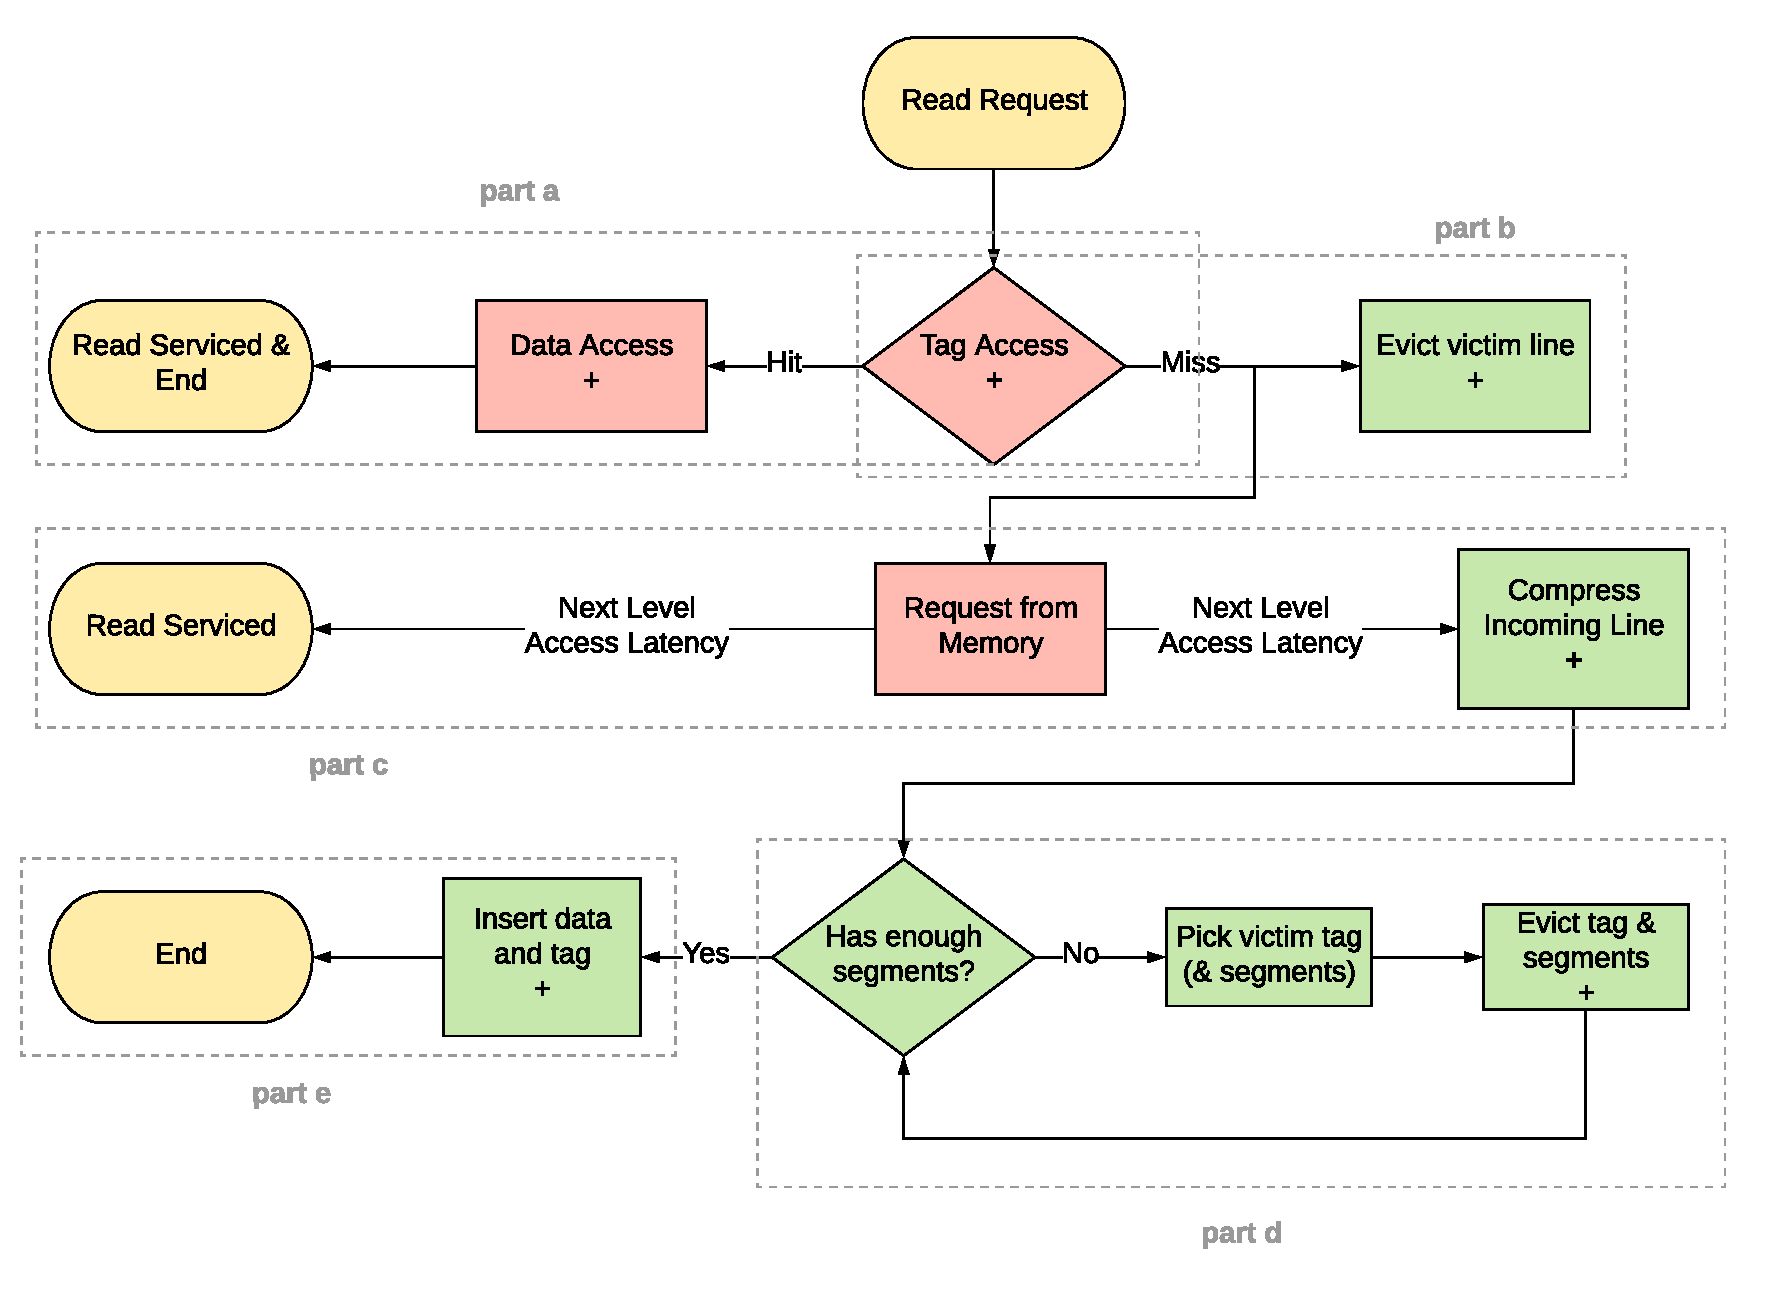
\includegraphics[width=\textwidth]{BDI_Read.pdf}
    \caption[BDI Read]{The flowchart shows the sequence of actions triggered by a read access to the BDI cache. Red blocks signify actions happening on the critical path, while green blocks mean actions happening off the critical path. Each + sign in any of the blocks signifies an extra latency for tag array access, data array access, or compression.}
    \label{fig:BDI_Read}
\end{figure}
\subsubsection{Cache Read}
A flowchart for the BDI cache read is shown in Figure \ref{fig:BDI_Read}. When the request first arrives the tag array is accessed. Part a in the figure shows the case when the tag access results in a hit, then the data line can be read, decompressed, and sent back to the requester right away. If the tag access is a miss, as shown in part b, a request is sent to the next cache level (or main memory), at the same time in parallel the replacement policy selects and evicts a tag. Once the requested line comes back from the next level it can be used to service the requester right away, inserting the line itself into the cache happens after that and off the critical path, as shown in part c.\par
So far through the access everything is similar to a conventional cache, Only the insertion of the new line is going to be different. The insertion of the new line starts in part c in the figure. Once the requested line comes back from next level, and in parallel to serving the requester, the line is BDI compressed. Then before the line is actually written to the cache we must verify that there is enough space in the data set for it. If there's not enough segments we have to trigger extra evictions in the current set to free up more segments, those evictions happen according to the tag replacement policy. The size caused evictions are shown in part d, and the line can finally be inserted once enough segments are available as shown in part e.\par
To avoid segmentation, the authors assume compaction always happens in the data array before each insertion, this is in accordance with previous work.
\begin{figure}[h]
    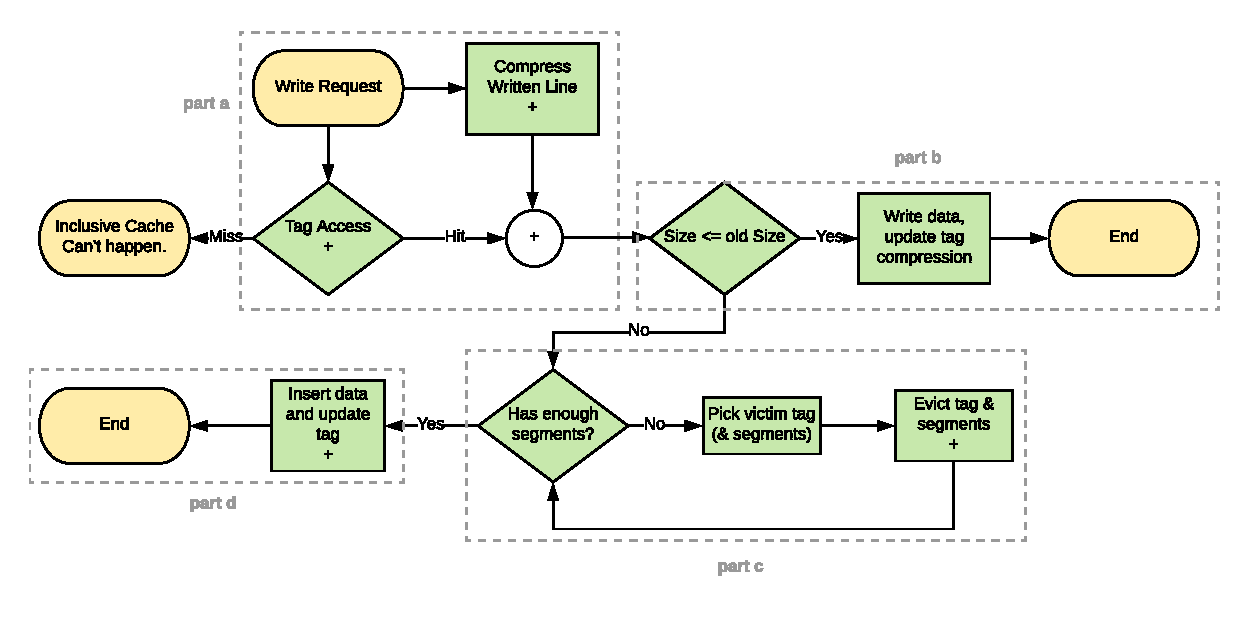
\includegraphics[width=\textwidth]{BDI_Write.pdf}
    \caption[BDI Write]{The flowchart shows the sequence of actions triggered by a write access to the BDI cache. All the blocks are shaded in green because any write request should be off the critical path of the processor regardless of it's status in the cache (hit or miss). Each + sign in any of the blocks signifies an extra latency for tag array access, data array access, or compression.}
    \label{fig:BDI_Write}
\end{figure}
\subsubsection{Cache Write}
A flowchart of write access to a BDI cache is shown in Figure \ref{fig:BDI_Write}. Because we always use inclusive caches, if a line is in a lower level cache it must also be in it's parent. A cache miss on a write request thus can never happen and a tag array access on a write request will always yield a hit as shown in part a. In parallel to the tag access, the written data line can also be compressed. Once we know the size of the compressed line, we can check whether or not it fits in it's old size, if it's the same or requires a lower number of segments, shown in part b, it can be written right away and the compression metadata in the tag array must also be updated. If the new compressed size is bigger than the old size, insertion of the new written line will trigger size based evictions, the replacement policy will be consulted for tags and their segments to be evicted until enough space for the new data line is free, this is shown in part c. Once there's enough segments the line can finally be written and it's tag's metadata can be updated accordingly as shown in part d.
As mentioned previously, the authors assume compaction always happens in the data array before each insertion, this is in accordance with previous work.

\section{Dedup}
\label{sec:Dedup}
\subsection{Structure}
\label{ssec:DedupStructure}
\subsubsection{Tag Array}
\label{sssec:DedupTag}
\subsubsection{Data Array}
\label{sssec:DedupData}
